\documentclass{article}

\usepackage[12pt]{extsizes}
\usepackage[T2A]{fontenc}
\usepackage[utf8]{inputenc}
\usepackage[english, russian]{babel}

\usepackage{mathrsfs}
\usepackage[dvipsnames]{xcolor}

\usepackage{amsmath}
\usepackage{amssymb}
\usepackage{amsthm}
\usepackage{indentfirst}
\usepackage{amsfonts}
\usepackage{enumitem}
\usepackage{graphics}
\usepackage{tikz}
\usepackage{tabu}
\usepackage{diagbox}
\usepackage{hyperref}
\usepackage{mathtools}
\usepackage{ucs}
\usepackage{lipsum}
\usepackage{geometry} % Меняем поля страницы
\usepackage{fancyhdr} % Headers and footers
\newcommand{\range}{\mathrm{range}}
\newcommand{\dom}{\mathrm{dom}}
\newcommand{\N}{\mathbb{N}}
\newcommand{\R}{\mathbb{R}}
\newcommand{\E}{\mathbb{E}}
\newcommand{\D}{\mathbb{D}}
\newcommand{\M}{\mathcal{M}}
\newcommand{\Prime}{\mathbb{P}}
\newcommand{\A}{\mathbb{A}}
\newcommand{\Q}{\mathbb{Q}}
\newcommand{\Z}{\mathbb{Z}}
\newcommand{\F}{\mathbb{F}}
\newcommand{\CC}{\mathbb{C}}

\DeclarePairedDelimiter\abs{\lvert}{\rvert}
\DeclarePairedDelimiter\floor{\lfloor}{\rfloor}
\DeclarePairedDelimiter\ceil{\lceil}{\rceil}
\DeclarePairedDelimiter\lr{(}{)}
\DeclarePairedDelimiter\set{\{}{\}}
\DeclarePairedDelimiter\norm{\|}{\|}

\renewcommand{\labelenumi}{(\alph{enumi})}

\newcommand{\smallindent}{
    \geometry{left=1cm}% левое поле
    \geometry{right=1cm}% правое поле
    \geometry{top=1.5cm}% верхнее поле
    \geometry{bottom=1cm}% нижнее поле
}

\newcommand{\header}[3]{
    \pagestyle{fancy} % All pages have headers and footers
    \fancyhead{} % Blank out the default header
    \fancyfoot{} % Blank out the default footer
    \fancyhead[L]{#1}
    \fancyhead[C]{#2}
    \fancyhead[R]{#3}
}

\newcommand{\dividedinto}{
    \,\,\,\vdots\,\,\,
}

\newcommand{\littletaller}{\mathchoice{\vphantom{\big|}}{}{}{}}

\newcommand\restr[2]{{
    \left.\kern-\nulldelimiterspace % automatically resize the bar with \right
    #1 % the function
    \littletaller % pretend it's a little taller at normal size
    \right|_{#2} % this is the delimiter
}}

\DeclareGraphicsExtensions{.pdf,.png,.jpg}

\newenvironment{enumerate_boxed}[1][enumi]{\begin{enumerate}[label*=\protect\fbox{\arabic{#1}}]}{\end{enumerate}}



\smallindent

\header{Математика}{\textit{Разное}}{6 класс}

%----------------------------------------------------------------------------------------

%\begin{document}\normalsize
\begin{document}
    \large

    \begin{center}
        \textbf{Разнобой}
    \end{center}


    \begin{enumerate_boxed}

        \item Сколько нужно сделать разрезов, чтобы разрезать 10 палок колбасы на 10 кусков каждую?

        \item После битвы со Змеем Горынычем три богатыря заявили:

        Добрыня Никитич: <<Это не я, это младшенький наш–Алешка.>>

        Илья Муромец: <<Я тут ни причем, это все Добрыня.>>

        Алеша Попович: <<Ну я, я убил!>>

        Кто убил змея, если только один из богатырей сказал правду?

        \item Можно ли a) квадрат $5 \times 5$ b) квадрат $5 \times 5$ c вырезанной угловой клеткой разрезать на доминошки?

        \item Сколько квадратов изображено на картинке ниже?

        \begin{table}[h]
            \centering
            \begin{tabular}{|c|c|c|c|}
                \hline
                \, & \, & \, & \, \\\hline
                &    &    &    \\\hline
                &    &    &    \\\hline
            \end{tabular}
            \label{tab:table}
        \end{table}

        \item В полосе из 11 клеток стоят два числа: в первой клетке число 6, а в девятой клетке число 4.
        Можно ли расставить числа в остальных клетках так, чтобы сумма чисел в любых трех подряд идущих клетках равнялась 15?
        \begin{figure}[h]
            \centering
            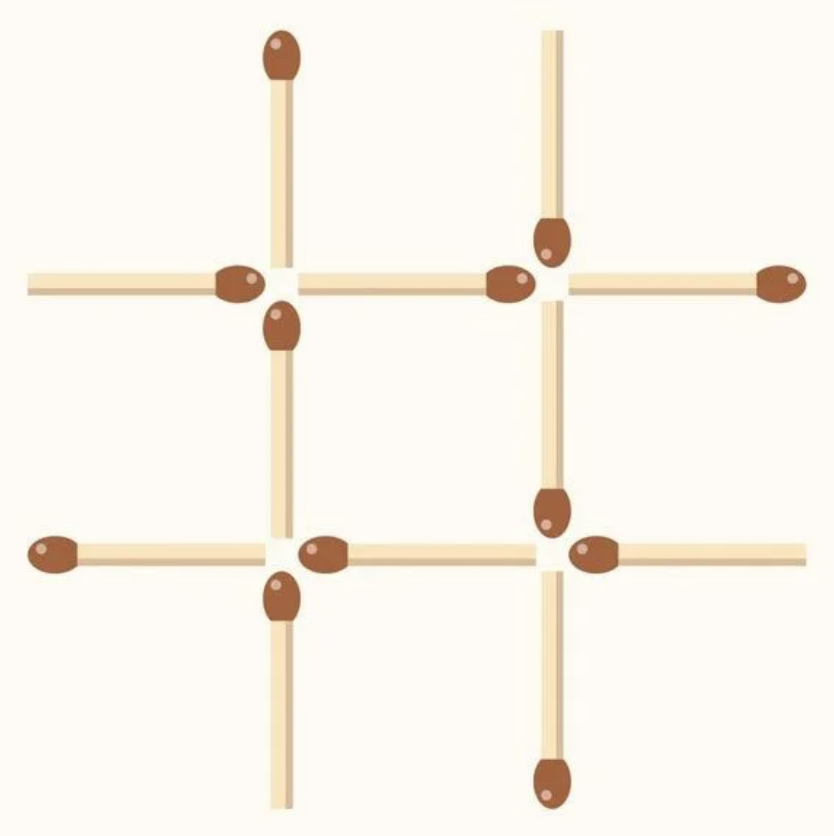
\includegraphics[width=0.3\linewidth]{spichki1}
            \caption{}
            \label{fig:figure3}
        \end{figure}
        \item Переложите 3 спички так, что бы на картинке~\ref{fig:figure3} получилось 3 квадрата.

        \item
        a) Три пирата делят слитки золота весом $1,2,\dots,10$ килограммов.
        Могут ли они поделить золото поровну, если распиливать слитки запрещается?

        b) При дележе один из пиратов был убит.
        Могут ли два оставшихся пирата разделить золото поровну, если распиливать слитки по-прежнему запрещается?

        \item Занятия кружка художественного свиста проходят по вторникам и четвергам.
        Оказалось, что в некотором месяце состоится 10 занятий этого кружка.
        На какой день недели приходится первое число этого месяца?

        \item Мистер Саша уверен, что можно вырезать из шахматной доски $8 \times 8$ ровно $4$ клетки так, чтобы оставшуюся доску можно было разрезать на “доминошки”, то есть прямоугольники $1 \times 2$.
        Прав ли Мистер Саша?

        \item Мистер Саша так понравилось вырезать из доски $8 \times 8$ четыре клетки и разбивать оставшуюся часть на доминошки, что теперь он уверен, что как ни вырежи $4$ клетки из шахматной доски $8 \times 8$, всегда оставшуюся фигурку можно разрезать на доминошки.
        Не ошибается ли Мистер Саша?


        \item Постройте отрицание к утверждениям:
        \begin{itemize}
            \item <<Поле шахматной доски - белое>>;

            \item <<Это или синее или белое>>;

            \item <<Я рыцарь или ты лжец>>;

            \item <<Верблюд синий и весит хотя бы 100 кг>>.
        \end{itemize}

        \item Сколько квадратов изображено на картинке ниже?

        \begin{table}[h]
            \centering
            \begin{tabular}{|c|c|c|c|c|}
                \hline
                \, & \, & \, & \, & \, \\\hline
                &    &    &    &    \\\hline
                &    &    &    &    \\\hline
                &    &    &    &    \\\hline
            \end{tabular}\label{tab:table2}
        \end{table}

        \item Найдите сумму a) $1+2+3+\dots+50;$ b) $1+2+3+\dots+51.$


        \item Получив двойку по географии, Вася решил порвать географическую карту в клочья.
        Каждый попавший ему в руки клочок он рвет на четыре части.
        Может ли он когда-нибудь получить ровно
        a) 2022 клочок?
        b) 2023 клочка?

        \item На прямой расположено пять точек $A, B, C, D, E$ (именно в таком порядке!).
        Известно, что $AB = 19$ см., $CE = 97$ см., $AC = BD$.
        Найдите длину отрезка $DE$.

        \item На каждой клетке доски $5 \times 5$ сидит один дрессированный лягушонок.
        По команде <<Ква!>> каждый лягушонок перепрыгивает на одну из соседних (по стороне) клеток.
        Докажите, что после команды <<Ква!>> какие-то два лягушонка окажутся на одной клетке.

        \item В кружке художественного свиста у каждого ровно один друг и ровно один враг.
        Докажите, что в кружке четное число людей.

        \item От шахматной доски $8 \times 8$ отрезали
        \begin{enumerate}
            \item угловую клетку (например, a1)

            \item две соседние угловые клетки (a1 и a8)

            \item две противоположные угловые клетки (a1 и h8).
        \end{enumerate}

        Можно ли оставшуюся часть разрезать на доминошки?

        \item Сколько квадратов изображено на картинке ниже?

        \begin{table}[h]
            \centering
            \begin{tabular}{|c|c|c|c|c|}
                \hline
                \, & \, & \, & \, & \, \\\hline
                &    &    &    &    \\\hline
                &    &    &    &    \\\hline
                &    &    &    &    \\\hline
                &    &    &    &    \\\hline
            \end{tabular}\label{tab:table3}
        \end{table}

        \item Четно или нечетно число $1^2 +2^2 +3^2 +\dotsc+100^2$

        \item Можно ли на шести книжных полках длиной по 1 м каждая расставить 150 книг, из которых a) 51; b) 50; c) 49 книг имеют толщину 6 см, а остальные – 3 см?

        \item Можно ли из семи прямоугольников $1 \times1, 1 \times2, 1 \times3, \dots, 1 \times6, 1 \times7$ сложить какой-нибудь прямоугольник, обе стороны которого больше 1?

        \begin{figure}[h]
            \centering
            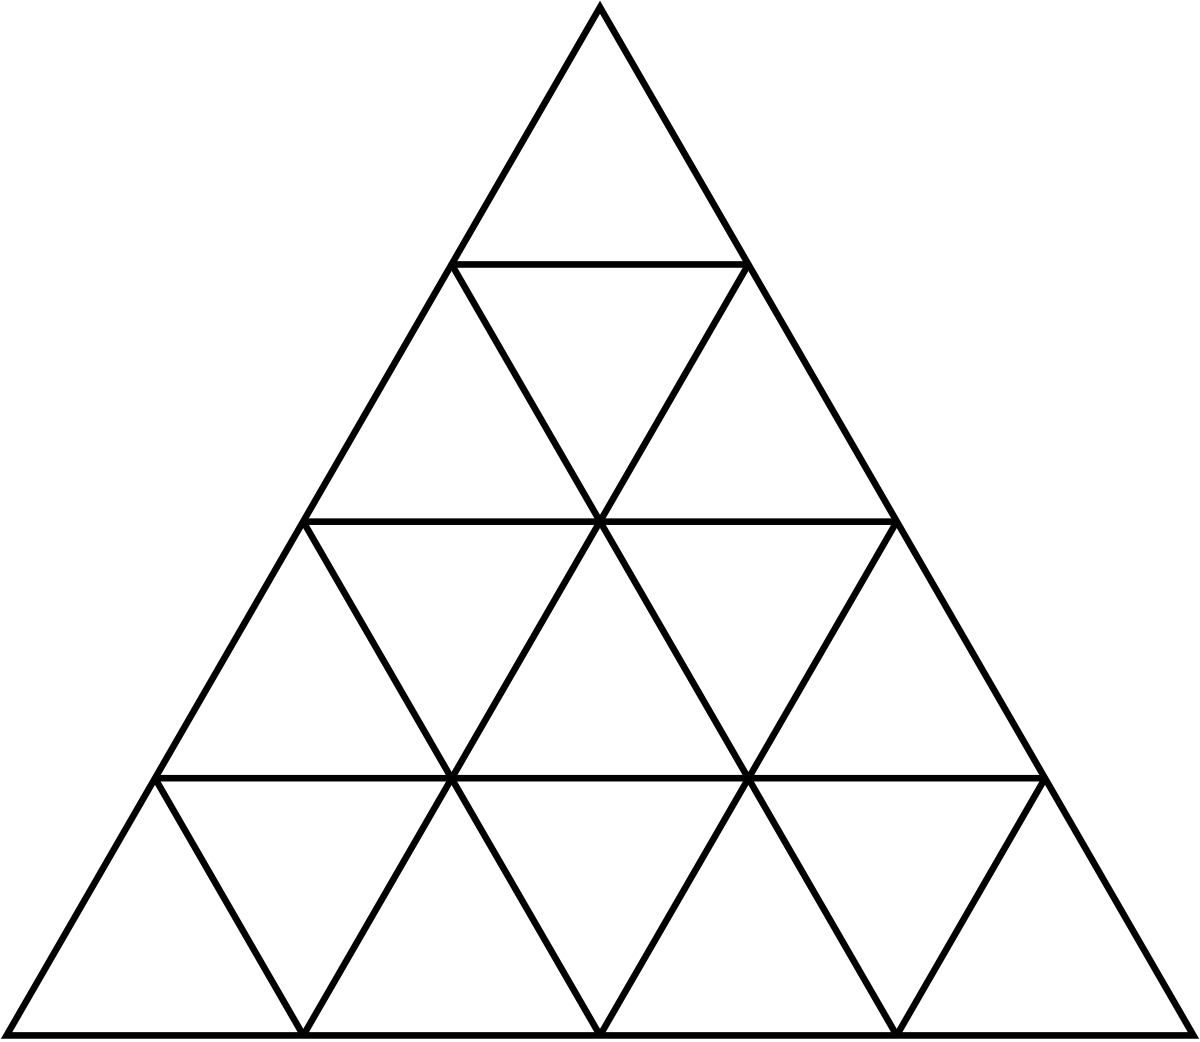
\includegraphics[width=0.3\linewidth]{triangle1}
            \caption{}
            \label{fig:triangle1}
        \end{figure}

        \item Сколько треугольников изображено на картинке~\ref{fig:triangle1}?

        \item Можно ли на шести книжных полках длиной по 1 м каждая расставить 150 книг, из которых a) 51; b) 50; c) 49 книг имеют толщину 6 см, а остальные – 3 см?

        \item В ковре размером $4 \times 4$ метра моль проела 15 дырок.
        Всегда ли можно вырезать коврик размером $1 \times 1$, не содержащий внутри дырок?
        (Дырки считаются точечными).

        \item Обязательно ли среди двадцати пяти монет достоинством 1, 2, 5 и 10 рублей найдётся семь монет одинакового достоинства?

        \item Докажите, что число

        \begin{enumerate}
            \item $4^{101} + 6^{101}$

            \item $9^{101} + 1$
        \end{enumerate}

        Делится на 10

        \item Сформулируйте и докажите:

        \begin{enumerate}
            \item Признак делимости на 2

            \item Признак делимости на 3

            \item Признак делимости на 5

            \item Признак делимости на 10

            \item Признак делимости на 6

            \item Признак делимости на 9

            \item Признак делимости на 4

            \item Признак делимости на 8
        \end{enumerate}

        \item Можно ли шашечную доску размером $10 \times 10$ замостить плитками размером $1 \times 4$?

        \begin{figure}[h]
            \centering
            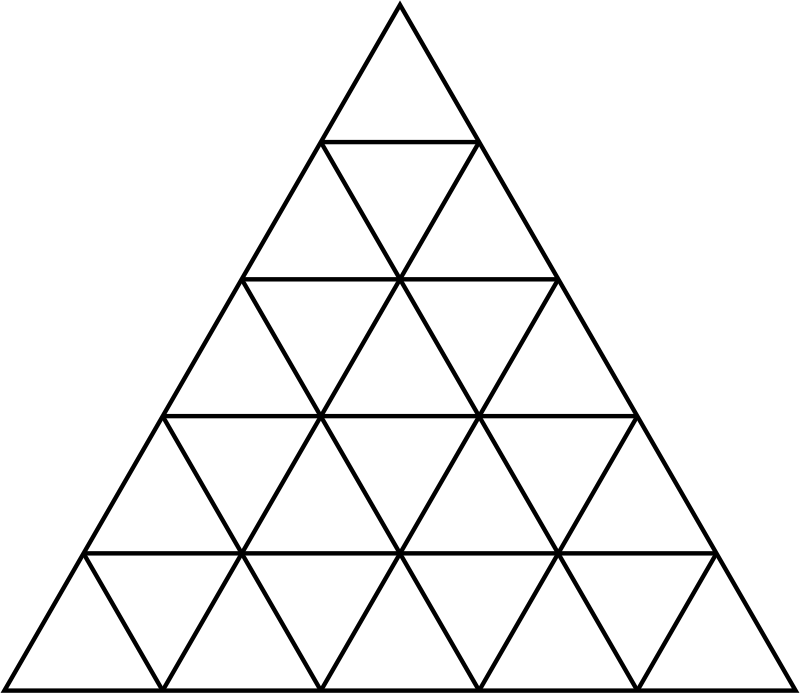
\includegraphics[width=0.3\linewidth]{triangle2}
            \caption{}
            \label{fig:triangle2}
        \end{figure}

        \item Сколько треугольников изображено на рисунке~\ref{fig:triangle2}?

        \item Можно ли из квадрата $7\times 7$ вырезать 10 квадратов $2\times2$?

        \item Треугольник разбит на треугольнички (25 штук), как показано на рисунке~\ref{fig:triangle2}.
        Жук может ходить по треугольнику, переходя между соседними (по стороне) треугольничками.
        Какое максимальное количество треугольничков может пройти жук, если в каждом он побывал не больше одного раза?

        \item Можно ли все клетки доски $9 \times 9$ обойти конём по одному разу и вернуться в исходную клетку?

        \item Можно ли доску размером $10 \times 10$ клеток разрезать на фигурки в форме буквы \texttt{T}

        \item На Васильевском острове 100 перекрёстков, и из каждого выходит ровно 4 дороги.
        А каждая дорога соединяет 2 перекрёстка.
        Сколько всего дорог на васильевском острове?

        \item В городе Калининград 15 телефонов.
        Можно ли их соединить проводами так, чтобы было четыре телефона, каждый из которых соединен с тремя другими, восемь телефонов, каждый из которых соединен с шестью, и три телефона, каждый из которых соединен с пятью другими?

        \item В стране Цифра есть 9 городов с названиями 1, 2, 3, 4, 5, 6, 7, 8, 9.
        Путешественник обнаружил, что два города соединены авиалинией в том и только в том случае, если двузначное число, составленное из цифр-названий этих городов, делится на 3.
        Можно ли добраться из города 1 в город 9?

        \item В кружке художественного свиста у каждого ровно один друг и ровно один враг среди членов кружка.
        Докажите, что кружок можно разделить на два кружка равной численности так, чтобы ни в одном из них не было ни друзей, ни врагов.

        \item 20 школьников решили 20 задач, причем каждую задачу решило ровно 2 школьника, и каждый школьник решил ровно 2 задачи.
        Докажите, что Тимофей Дмитриевич может организовать разбор так, чтобы каждая задача была рассказана ровно по одному разу, а каждый школьник рассказал ровно одну из решенных им задач.

        \item Докажите, что из любых трех натуральных чисел можно выбрать два, разность которых делится на 2

        \item Докажите, что из любых четырёх натуральных чисел можно выбрать два, разность которых делится на 3

        \item Найдите остаток от деления $2^{100}$ на 3.

        \item Можно ли монетами по 14 и 35 шиллингов заплатить без сдачи сумму в 2024 шиллингов?

        \item Гидрометцентр сообщает, что в 2023 году в Санкт-Петербурге пасмурных дней было в 5 раз больше, чем солнечных.
        Докажите, что Гидрометцентр ошибается.

        \item Может ли сумма трёх последовательных натуральных чисел быть простым числом?

        \item Какое из чисел больше: $2^{30}$ или $3^{20}$?

        \item Делится ли число 32561698 на 12?
        Решите эту задачу:
        \begin{enumerate}
            \item с помощью признака делимости на 4;
            \item с помощью признака делимости на 3.
        \end{enumerate}

        \item Даша и Таня по очереди выписывают на доску цифры шестизначного числа.
        Сначала Даша выписывает первую цифру, затем Таня — вторую, и так далее.
        Таня хочет, чтобы полученное в результате число делилось на три, а Даша хочет ей помешать.
        Кто из них может добиться желаемого результата независимо от ходов соперника?

        \item Замените звездочки в записи числа 72*4* цифрами так, чтобы это число делилось на 45.
        Укажите все возможные варианты!

        \item
        \begin{enumerate}
            \item Докажите, что произведение двух последовательных чётных чисел всегда делится на 8.

            \item Может ли произведение четырех последовательных натуральных чисел оканчиваться на 116?

        \end{enumerate}


        \item Может ли натуральное число, записываемое с помощью 10 нулей, 10 единиц и 10 двоек, быть квадратом некоторого другого натурального числа?

        \item Сколько существует натуральных чисел меньших 1000 и таких, что произведение всех цифр числа равно 6?

        \item Серия для шестиклассников, выданная на первом занятии январской математической смены, состоит из 7 задач.
        Из 16 ребят каждый сдал больше половины серии.
        Докажите, что какую-то задачу решило не менее 10 человек.

        \item Найдите последнюю цифру числа $7^{49}$.


        \item Одним взмахом меча Богатырь И.
        Муромец может отсечь З.
        Горынычу одну голову или сразу 10 голов (конечно, если их было не меньше 10).
        Однако, если после отсечения осталось чётное число голов, то число голов сразу же удваивается.
        Изначально, у З.
        Горыныча 444 головы.
        Может ли Богатырь отрубить З.
        Горынычу все его головы?

        \item Вова забыл номер телефона ($8\,931\star\star\star\star\star\star\,\star$) своей девушки Маши, но помнит, что дальше в нем были только девятки и двойки, причем двоек было больше, чем девяток.
        Также он вспомнил, что номер (как 11-значное число) делился на три и на четыре.
        Помогите Вове вспомнить номер Маши.

        \item Ы и Ь --- только такие две буквы есть в алфавите некоторого племени.
        Каждая конечная последовательность из этих букв является словом и что-то да значит.
        От замен следующих буквосочетаний в словах смысл слова не меняется: ЫЫЬ\,$\Leftrightarrow$\,ЬЬ, ЬЫЫ\,$\Leftrightarrow$\,ЫЬЫ, ЬЫЬ\,$\Leftrightarrow$\,ЫЬ, ЬЬЬ\,$\Leftrightarrow$\,ЫЫ (замену можно делать в любом месте слова).
        Обязательно ли смысл у слов ЫЬЫ и ЬЫЬ одинаков?

        \item Могут ли все три числа $a, b, c$ быть меньше $-1$, если известно, что \[ab+a+b = c?\]

        \item Гриша вычислил сумму первых 2024 чисел из ряда $9, 99, 999, \ldots$.
        Сколько различных цифр содержит результат?

        \item Олег лёг спать в 10 вечера и завел будильник (со стрелками и~циферблатом на 12 делений) на 7 утра.
        Ночью в некоторый момент будильник, до этого работавший исправно, сломался, и его стрелки пошли в обратную сторону (с прежней скоростью).
        Тем не менее, утром будильник прозвенел точно в положенное время.
        Во сколько сломался будильник?

        \item Докажите, что из чисел $x+y-2z$, $x+z-2y$, $y+z-2x$ хотя бы одно неотрицательно.

        \item Одно утверждение среди следующих неверно.
        Найдите его:

        - если точный квадрат делится на 6, то он делится на 36;

        - если точный квадрат делится на 7, то он делится на 49;

        - если точный квадрат делится на 8, то он делится на 64.

        \item Максим отметил несколько клеток в квадрате $12 \times 12$ так, что в любом a) прямоугольнике $1 \times 3$; b) $L$--тетрамино есть отмеченная клетка.
        Какое наименьшее число клеток мог отметить Максим?

        \item Проверь свою наблюдательность.
        В условиях задач скрыто некоторое \emph{послание}.
        Какое?

        \item Петя перемножил натуральные числа от 1 до 20.
        На сколько нулей оканчивается полученное произведение?

        \item Петя перемножил натуральные числа от 1 до 30.
        На сколько нулей оканчивается полученное произведение?

        \item Про каждое из следующих чисел скажите, является ли оно простым: 0, 1, 12, 13, 17, 97, 899, 43825539123, 621212229, 100020001.
        Обоснуйте каждый свой ответ.

        \item В ряд выписаны числа от 1 до 25.
        Можно ли расставить между
        ними знаки <<+>> и <<-->> так, чтобы значение полученного выражения
        было равно нулю?

        \item Имеется много одинаковых квадратов.
        В вершинах каждого из них в произвольном порядке написаны числа 1, 2, 3 и 4.
        Квадраты сложили в стопку и написали сумму чисел, попавших в каждый из четырех углов стопки.
        Может ли оказаться так, что в каждом углу стопки сумма равна $2024$?


        \item Может ли число, десятичная запись которого состоит из 2024 нулей, 2024 единиц и 2024 двоек, быть точным квадратом?


        \item Найдите наибольшее четырёхзначное число, все цифры которого различны и которое делится на 2, 5, 9 и 11.

        \item При каких простых $p$ число $5p + 1$ тоже простое

        \item Можно ли разменять 100 фертингов монетами по 1, 3, 5 и 25 фертингов так, чтобы всего оказалось 33 монеты?

        \item На доске написано 1012 плюсов и 1013 минусов.
        За один ход разрешается стереть любые два знака и написать вместо них плюс (если они одинаковы) или минус (если они различны).
        Какой знак останется на доске через 2024 ходов?

        \item В каждой клетке таблицы $2023\times2023$ написано целое число.
        Оказалось, что сумма чисел в каждой строке нечётна.
        Докажите, что сумма чисел в каком-то столбце таблицы также нечётна.

        \item Разложите на простые множители число 4704.

        \item Разложите на простые множители число 899.

        \item Может ли произведение числа и суммы его цифр равняться 4704?

        \item Натуральное число умножили на произведение всех его цифр.
        Получилось 1995.
        Найдите исходное число.

        \item Найдите $n$ из равенства $5^{47} \cdot 5^{19} = 5^n$.

        \item Вася возводил число в квадрат и получил 1234567.
        Его друг Петя сказал: <<Пересчитай, а то получишь двойку>>.
        Докажите, что Петя прав.

        \item На острове живут рыцари, которые всегда говорят правду, и лжецы, которые всегда лгут.
        На улице встретились два жителя острова.
        Один из них сказал: <<По крайней мере один из нас рыцарь>>.
        Второй ему ответил: <<Ты лжец>>.
        Кто из них кто?

        \item Можно ли в выражении $1 * 2 * 3*4*5*6*7*8*9$ заменить все звездочки на $+$ или $-$ так, чтобы в ответе получилось
        a) 1?
        b) 0?

        \item Разложите 2008 на простые множители

        \item Число умножили на его сумму цифр и получили 2008.
        Найдите все такие числа.

        \item Разложите 2017 на простые множители

        \item Вася возводил число в квадрат и получил 1234567.
        Его друг Петя сказал: <<Пересчитай, а то получишь двойку>>.
        Докажите, что Петя прав.

        \item Сумма двух чисел 627.
        Одно число заканчивается нулём.
        Если это нуль зачеркнуть, то получится второе число.
        Найди эти числа.

        \item Котят было на 6 больше, чем цыплят, а ног все котята имели на 44 больше, чем все цыплята.
        Сколько было котят?

        \item Маша съела половину всех конфет и ещё одну, а Даша - половину остатка, и ещё осталось 5 конфет.
        Сколько конфет съела Маша?

        \item Расставьте по кругу цифры от 1 до 9, каждую по одному разу, так, чтобы каждое двузначное число, составленное из двух идущих подряд по часовой стрелке цифр, делилось на 3 или 4.

        \item Тане и Ване дали одинаковые многоугольники из бумаги.
        Таня отрезала от своего листа кусок, и остался квадрат.
        Ваня отрезал точно такой же (и по форме, и по размеру) кусок по-другому, и у него остался треугольник.
        Нарисуйте пример, как это могло быть.

        \item  Каждая клетка доски $10 \times 10$ покрашена в синий или белый цвет.
        Назовём клетку радостной, если ровно две соседних с ней клетки синие.
        Закрасьте доску так, чтобы все клетки были радостными.
        (Клетки считаются соседними, если имеют общую сторону.)

        \item На доске записано натуральное число.
        Каждую минуту с ним делают следующую операцию: если в нём есть две одинаковых цифры, то стирают любую из них; если же все цифры различны, то стирают всё число и вместо него пишут втрое большее число.
        Например, из числа 57 можно за две минуты получить $57 \rightarrow 171 \rightarrow 71$ или $57 \rightarrow 171 \rightarrow 17$.
        Мария написала двузначное число и через несколько минут снова получила его же.
        Приведите пример, как она могла это сделать.

        \item Вершины правильного 222-угольника покрасили в красный и синий цвет.
        Будем называть сторону одноцветной, если вершины покрашены в один цвет, и разноцветной, если они покрашены в разные цвета.
        Можно ли так раскрасить вершины, чтобы одноцветных и разноцветных сторон было поровну?
    \end{enumerate_boxed}
\end{document}